\chapter{Návrh}

\subsection{Koncept riešenia}

\hspace{10mm}Pri návrhu nášho riešenia sa zameriame na metódy učenia s učiteľom pomocou hlbokých neurónových sietí. Náš model bude pozostávať s konvolučnej neurónovej siete, pričom hlavný dôraz bude na tvorenie filtrov v prvých vrstvách. Porovnáme rôzne typy a techniky na tvorenie filtrov, ako sú automatické filtre, teda také, ktoré si sieť vytvorí sama, a manuálne, ktoré bude sieť čítať z externého súboru. Nakoniec vyhodnotíme najlepší spôsob vytváranie filtrov na základe dosiahnutých presností jednotlivých sietí. Budeme pritom zohľadňovať aj množstvo dát, ktoré jednotlivé siete budú potrebovať a čas trénovania. Naša konvolučná neurónová sieť bude mať za úlohu klasifikovať histologické dáta, konkrétne histologické dáta rakoviny prsníka. Klasifikovať budeme na dve kategórie a to pozitívna rakovina prsníka a negatívna rakovina prsníka. 

\subsubsection*{Konvolučná neurónová sieť s back propagation}
\hspace{10mm}Prvý typ neurónovej siete, ktorý vytvoríme, bude klasická konvolučná neurónová sieť, kde sa filtre budú vytvárať automaticky a to jednoduchým použitím techniky back propagation. 

\subsubsection*{Gáborové filtre}
\hspace{10mm}Druhý typ konvolučnej neurónovej siete, ktorý vytvoríme, bude vytváranie filtrov manuálne, teda sieť si ich nebude inicializovať sama,  ani ich nebude upravovať pomocou učenia, ale bude ich čítať z externého súboru. Do tohto súboru pridáme filtre, pričom na ich výrobu využijeme Gáborovú funkciu, teda použijeme Gáborové filtre, ktorých opis nájdeme v odstavci \ref{gaborfilter}. Iná možnosť je, že ich nebudeme čítať z externého súboru, ale budeme ich vytvárať priamo v sieti, ale len pomocou Gáborovej funkcie, nebude možnosť ich „vylepšovať”.

\subsubsection*{Autoenkóder}
\hspace{10mm}Ďaľší typ konvolučnej neurónovej siete bude autoenkóder, pomocu ktorého budeme vytvárať filtre. Celková myšlienka autoenkóderu je opísaná v časti \ref{autoenkoder}. Túto metódu použijeme takým spôsobom, že autoenkóderom sa budeme snažiť skopírovať a následne prekopírovať jednotlivé dáta. Po dokončení tejto úlohy, teda natrénovaní autoenkóderu na dátach, tieto hodnoty skopírujeme a využijeme v tvorení filtrov. Následne túto vrstvu odstránime a uložíme filtre. Tento spôsob sa radí medzi automatické vytváranie filtrov, pretože budú výsledkom učenia siete na dátach. Vďaka týmto filtrom budeme ďalej vykonávať úlohu klasifikácie nad spomínanými dátami pomocu klasickej konvolučnej neurónovej siete.

\subsubsection*{Transfer learning}
\hspace{10mm}Posledný typ konvolučnej neurónovej siete, ktorý budeme vytvárať, je vytváranie filtrov pomocou Transfer learningu, ktorého princíp je opísaný v časti \ref{transferlearning}. My však nebudeme používať už vytvorenú konvolučnú neurónovú sieť, ale budeme si ju vytvárať samy. Najskôr teda vytvoríme konvolučnú neurónovú sieť, ktorú budeme trénovať na inom datasete. Následne túto sieť upravíme, odstránime niektoré jej natrénované váhy a využijeme filtre, ktoré si vytvorila. Takto upravenú sieť budeme tiež trénovať na hlavnom datasete, a nakoniec vykonáme klasifikáciu na validačnom datasete.  

\subsection{Opis datasetu}
\hspace{10mm}Jednou z hlavných častí návrhu sú aj dáta, ktoré sa budú používať pre riešenie. Hlavným zdrojom dát pre naše riešenie bude stránka grand-challenge.org a konkrétne súťaž ECDP2020. Tento dataset obsahuje 360 výrezov histologických dát rakoviny prsníka, kde 114 je na túto rakovinu pozitívnych a 216 ich je negatívnych. Testovacie dáta budú k dispozícii v januári 2020. Tieto dáta sú vo formáte MIRAX, ktorý sa používa na ukladanie medicínskych dát s veľkou veľkosťou. Veľkosť celého datasetu je 755 GB a jednotlivé obrazy výrezov nie je možné prehliadať vo väčšine softvérov, odporúča sa softvér CaseViewer. Táto súťaž sa zaoberá klasifikáciou rakoviny prsníka konkrétne HER2 transmembránového proteínu, ktorý je bližšie opísaný v časti \ref{HE2protein}. (Obrázok \ref{fig:dataseUkazka})

\begin{figure}[h!]
\begin{centering}
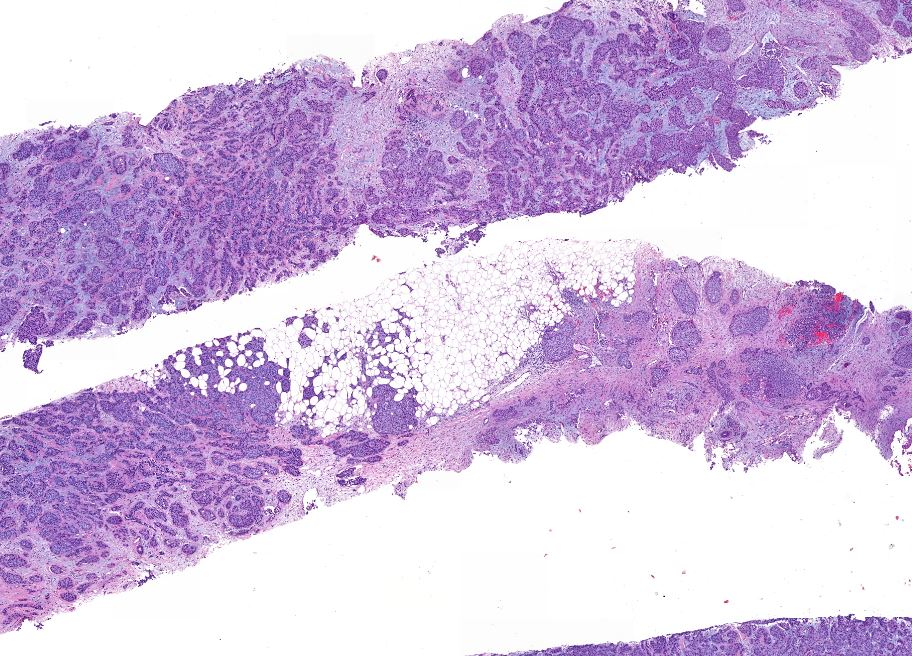
\includegraphics[width=15cm]{assets/images/300_1.JPG}
\par\end{centering}
\caption{Ukážka dataset ECDP2020. \label{fig:dataseUkazka}\cite{ECDP2020}}
\end{figure}

\hspace{10mm}Vedľajším zdrojom dát bude súťaž s menom PatchCamelyon, ktorá obsahuje 327 680 histologických dát, ktoré sú extrahované z lymfatických buniek. Jednotlivé obrazy sú vo veľkosti 96x96 pixelov. Tento dataset bude slúžiť hlavne ako trénovací dataset pre úlohu, v ktorej budeme vytvárať filtre pomocou Transfer learning-u



% \hspace{10mm}

% \say{Here, a quotation is written and even some \say{nested} quotations 
% are possible}

% Figure \ref{fig:dynabook}:

% \begin{figure}[h!]
% \begin{centering}
% \includegraphics[width=10cm]{assets/images/Dynabook}
% \par\end{centering}
% \caption{Dynabook \label{fig:dynabook}}
% \end{figure}
